\subsubsubsection{Rede neural convolucional}

Uma rede neural convolucional é análoga à rede neural artificial, isto é, é feita de neurônios que otimizam o aprendizado por meio deles mesmos. A principal diferença é que a rede neural convolucional é amplamente utilizada em soluções que detectam padrões em imagens. Portanto, existem funcionalidades específicas da própria arquitetura voltadas para essa tarefa \space\cite{oshea2015introduction}.

A arquitetura básica de uma rede neural convolucional possui as seguintes camadas: convolucional, de agrupamento e totalmente conectada, conforme ilustrado na \cref{fig:arquitetura_cnn} \space\cite{dp_overview}.

\begin{figure}[ht]
\caption{Camadas principais de uma rede neural convolucional}
\centering % para centralizarmos a figura
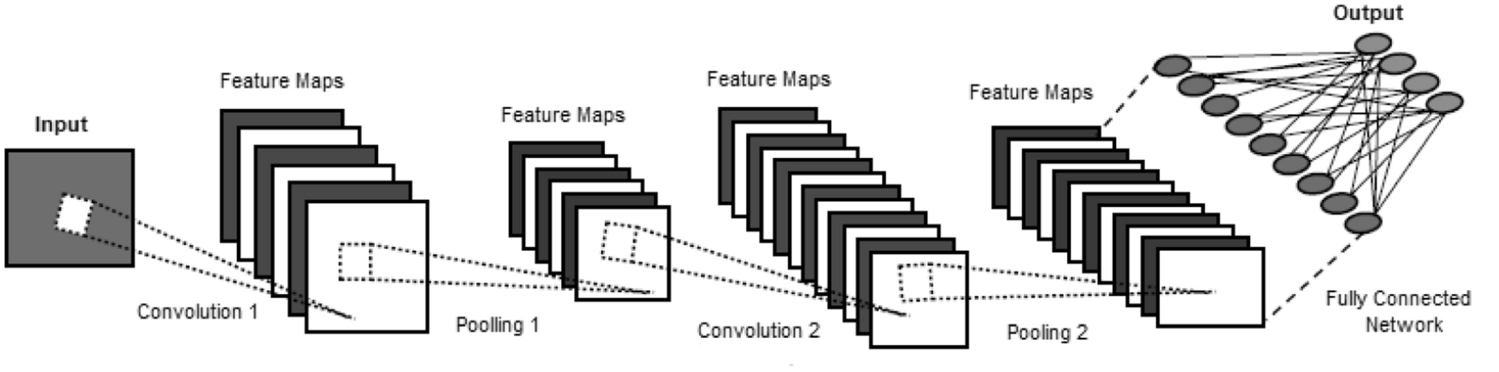
\includegraphics[width=15cm]{figures/arquitetura_cnn.png} % leia abaixo
\legend{Fonte: \citeonline{dp_overview}}
\label{fig:arquitetura_cnn}
\end{figure}

\subsubsubsection*{Camada convolucional}

Conforme descrito por \citeonline{computation11030052}, a camada convolucional é essencial para esse tipo de arquitetura. Ela utiliza um filtro — ou kernel — que é aplicado na imagem e direcionado para o próximo neurônio. Esse filtro é uma matriz de números que realiza uma operação em todos os pixels da imagem — também representada por matriz(es) —. As informações cruciais para esse filtro são: tamanho, largura e pesos. Essa abordagem é utilizada para extrair características com uma base matemática, criando uma relação direta entre um pixel e os pixels ao seu redor. Os pesos começam de forma pseudoaleatória e são ajustados ao longo do aprendizado. O resultado dessa camada é chamado de mapa de características. O tamanho da saída é baseado na fórmula abaixo, considerando os tamanhos I da imagem, F do filtro e S da saída \space\cite{computation11030052}.

\begin{gather}
    \mathbf{I}x - \mathbf{F}x + 1 = \mathbf{S}x \notag \\
    \mathbf{I}y - \mathbf{F}y + 1 = \mathbf{S}y
\end{gather}


A seguir um exemplo dos passos para construir a matriz resultante baseado em \citeonline{Alzubaidi2021}.

\clearpage

$$
\hspace{0.4cm}
\begin{tikzpicture}[baseline=(M.center)]
 \matrix (M) [matrix of math nodes,left delimiter={[},right delimiter={]}] {
 0 & 2 & 1 & 0 \\
 1 & 0 & 0 & 1 \\
 };
 \draw (M-1-1.north west) rectangle (M-2-2.south east);
 \node[above=10pt of M.north] {Matriz 2x4};
\end{tikzpicture}
\hspace{0.8cm}\bigotimes\hspace{0.8cm}
\begin{tikzpicture}[baseline=(M.center)]
 \matrix (M) [matrix of math nodes,left delimiter={[},right delimiter={]}] {
  0 & 1 \\
 -1 & 2 \\
 };
 \node[above=10pt of M.north] {Filtro 2x2};
\end{tikzpicture}
\hspace{0.8cm}=\hspace{0.8cm}
\begin{tikzpicture}[baseline=(M.center)]
 \matrix (M) [matrix of math nodes,left delimiter={[},right delimiter={]}] {
    \boxed{1} & - & - \\
 };
 \node[above=10pt of M.north] {Resultado};
\end{tikzpicture}
$$

$$
\begin{tikzpicture}[baseline=(M.center)]
 \matrix (M) [matrix of math nodes,left delimiter={[},right delimiter={]}] {
    0 & 2 & 1 & 0 \\
    1 & 0 & 0 & 1 \\
 };
 \draw (M-1-2.north west) rectangle (M-2-3.south east);
\end{tikzpicture}
\hspace{0.8cm}\bigotimes\hspace{0.8cm}
\begin{tikzpicture}[baseline=(M.center)]
 \matrix (M) [matrix of math nodes,left delimiter={[},right delimiter={]}] {
  0 & 1 \\
  -1 & 2 \\
 };
\end{tikzpicture}
\hspace{0.8cm}=\hspace{0.8cm}
\begin{bmatrix}
 1 & \boxed{1} & - \\
 \end{bmatrix}
$$

$$
\hspace{0.2cm}
\begin{tikzpicture}[baseline=(M.center)]
 \matrix (M) [matrix of math nodes,left delimiter={[},right delimiter={]}] {
    0 & 2 & 1 & 0 \\
    1 & 0 & 0 & 1 \\
 };
 \draw (M-1-3.north west) rectangle (M-2-4.south east);
\end{tikzpicture}
\hspace{1cm}\bigotimes\hspace{0.9cm}
\begin{tikzpicture}[baseline=(M.center)]
 \matrix (M) [matrix of math nodes,left delimiter={[},right delimiter={]}] {
  0 & 1 \\
  -1 & 2 \\
 };
\end{tikzpicture}
\hspace{0.8cm}=\hspace{0.8cm}
\begin{bmatrix}
 1 & 1 &  \boxed{2} \\
 \end{bmatrix}
$$

\subsubsubsection*{Tamanho do passo e preenchimento}

O tamanho do passo — ou \textit{stride} — é usado para especificar a distância, em pixels, entre os passos da camada. No exemplo mencionado anteriormente, esse parâmetro é definido como 1, o que significa que a matriz selecionada avança 1 pixel para a direita a cada passo. Esse valor altera o tamanho da matriz resultante \space\cite{dp_overview}.

O preenchimento — ou \textit{padding} — é uma técnica empregada para manter o mesmo tamanho da entrada, adicionando bordas com zeros antes das operações da camada. Isso resulta em uma matriz de saída com a mesma dimensão da matriz original. A técnica é utilizada para evitar a perda de detalhes nas bordas das imagens durante o processamento de uma camada \space\cite{dp_overview}.

\subsubsubsection*{Camada de agrupamento}

A camada de agrupamento — ou \textit{pooling} — tem como função primordial reduzir o tamanho do mapa de características, preservando, contudo, os padrões mais relevantes. Entre os aspectos essenciais dessa camada estão o tamanho do agrupamento e a operação a ser realizada. Um dos principais problemas dessa camada é que ela identifica apenas a presença e a localização das características, sem preservá-las integralmente. Dependendo da operação escolhida e do número de camadas, isso pode resultar em perda de características importantes, afetando negativamente o desempenho final da predição \space\cite{dp_overview}.

Existem vários tipos de agrupamento, sendo os mais comuns o agrupamento máximo, o agrupamento médio e o agrupamento global médio. Esses tipos são explicados abaixo, com exemplos baseados em \citeonline{Alzubaidi2021}.

\subsubsubsection*{Agrupamento máximo}

Esta técnica define o resultado com base no valor máximo encontrado dentro do tamanho do agrupamento. Um exemplo pode ser ilustrado utilizando um mapa de características de tamanho 4x4 e um agrupamento de tamanho 2x2.

$$
\begin{tikzpicture}[baseline=-0.5ex]
    \matrix (M) [matrix of math nodes,left delimiter={[},right delimiter={]}] {
        4 & 25 & 44 & 10\\
        8 & 14 & 8 & 33 \\
        17 & 2 & 16 & 34 \\
        5 & 13 & 24 & 7 \\
    };
    \draw (M-1-1.north west) rectangle (M-2-2.south east);
\end{tikzpicture}
=
\begin{bmatrix}
	\boxed{25} & 44 \\
	17 & 34 \\
   \end{bmatrix}
$$

\subsubsubsection*{Agrupamento médio}

Neste método, o resultado é definido com base na média dos valores encontrados dentro do tamanho do agrupamento. Um exemplo pode ser ilustrado utilizando um mapa de características de tamanho 4x4, com um agrupamento de tamanho 2x2. Esse processo calcula a média dos valores em cada janela de agrupamento de 2x2, gerando uma matriz de saída reduzida que preserva as informações médias das características originais.

$$
\begin{tikzpicture}[baseline=-0.5ex]
    \matrix (M) [matrix of math nodes,left delimiter={[},right delimiter={]}] {
        4 & 25 & 44 & 10\\
        8 & 14 & 8 & 33 \\
        17 & 2 & 16 & 34 \\
        5 & 13 & 24 & 7 \\
    };
    \draw (M-1-1.north west) rectangle (M-2-2.south east);
\end{tikzpicture}
=
\begin{bmatrix}
	\boxed{12} & 23 \\
	9 & 20 \\
   \end{bmatrix}
$$

\subsubsubsection*{Agrupamento global médio}

Neste método, o resultado é obtido pela média geral do mapa de características, o que resulta, invariavelmente, em uma matriz de saída de dimensão 1x1. Por exemplo, considerando um mapa de características de tamanho 4x4, o agrupamento global médio calculará a média de todos os valores presentes neste mapa, condensando toda a informação em um único valor representativo. Essa abordagem é particularmente útil para reduzir significativamente as dimensões dos dados, mantendo uma representação global das características essenciais.

$$
\begin{tikzpicture}[baseline=-0.5ex]
    \matrix (M) [matrix of math nodes,left delimiter={[},right delimiter={]}] {
        4 & 25 & 44 & 10\\
        8 & 14 & 8 & 33 \\
        17 & 2 & 16 & 34 \\
        5 & 13 & 24 & 7 \\
    };
\end{tikzpicture}
=
\begin{bmatrix}
	16
   \end{bmatrix}
$$

\subsubsubsection*{Camada totalmente conectada}

A camada totalmente conectada é geralmente utilizada no final da arquitetura. Ela estabelece uma ligação direta de cada neurônio a cada etiqueta final, tornando essa camada extremamente pesada em termos computacionais. O número de neurônios nesta camada é equivalente ao número de classes propostas. Além disso, é nesta camada que a função de perda é calculada, iniciando o processo de retropropagação \space\cite{Alzubaidi2021, computation11030052}.

\subsubsubsection*{Aperfeiçoamento}

De acordo com \citeonline{Alzubaidi2021, computation11030052}, existem várias técnicas para aperfeiçoar os resultados do modelo, incluindo:

\begin{itemize}
\item Dropout: Esta técnica é amplamente utilizada para evitar o sobreajuste. Ela desativa aleatoriamente um neurônio durante o treinamento, forçando o modelo a aprender a identificar características em outros neurônios, o que possibilita a generalização do modelo.
\item Aumentar o tamanho do conjunto de dados: Se não for possível obter um conjunto de dados maior, técnicas de aumento artificial podem ser empregadas, como rotacionar, recortar e inverter as imagens horizontal ou verticalmente.
\item Normalização em lote: Esta técnica normaliza as saídas para acelerar o treinamento da rede.
\item Aumentar o tempo de treinamento.
\item Aumentar a profundidade ou largura da arquitetura.
\item Ajustar os hiperparâmetros.
\end{itemize}
